\documentclass[10pt]{beamer}
\usepackage{uglixbeamer,animate}
\title{Autres types de graphes}
\subtitle{Chapitre 21}
\author{NSI2}

\begin{document}
\maketitle

\section{Graphes non orientés}

\begin{frame}{Situation}
Pour faire simple, dans un graphe non orienté il n'y a pas d'arc dirigé d'un sommet vers l'autre, simplement une arête reliant les deux sommets !

\begin{center}
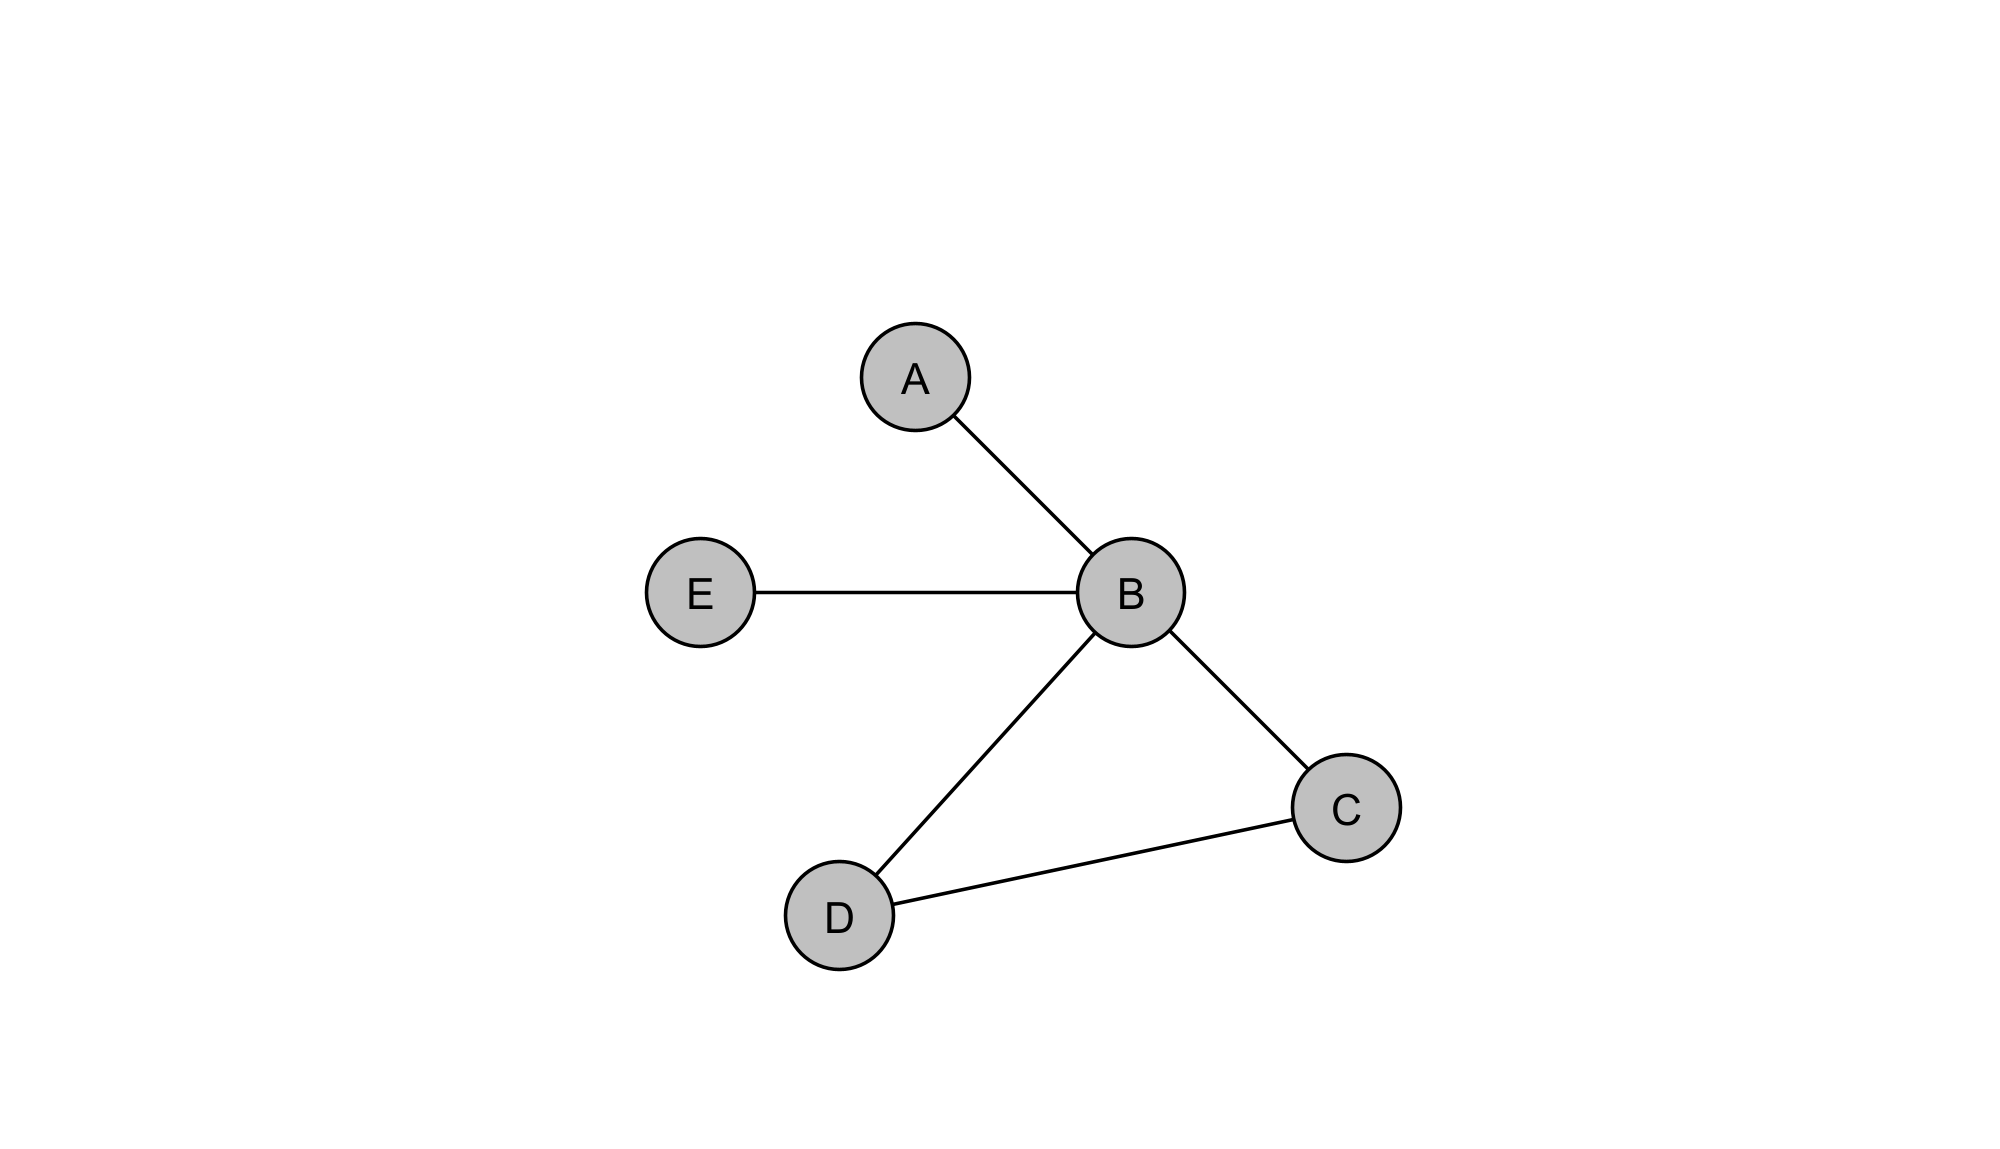
\includegraphics[width=9cm]{img/graph1}
\end{center}
\end{frame}
\begin{frame}{Vocabulaire}
\begin{center}
\only<1>{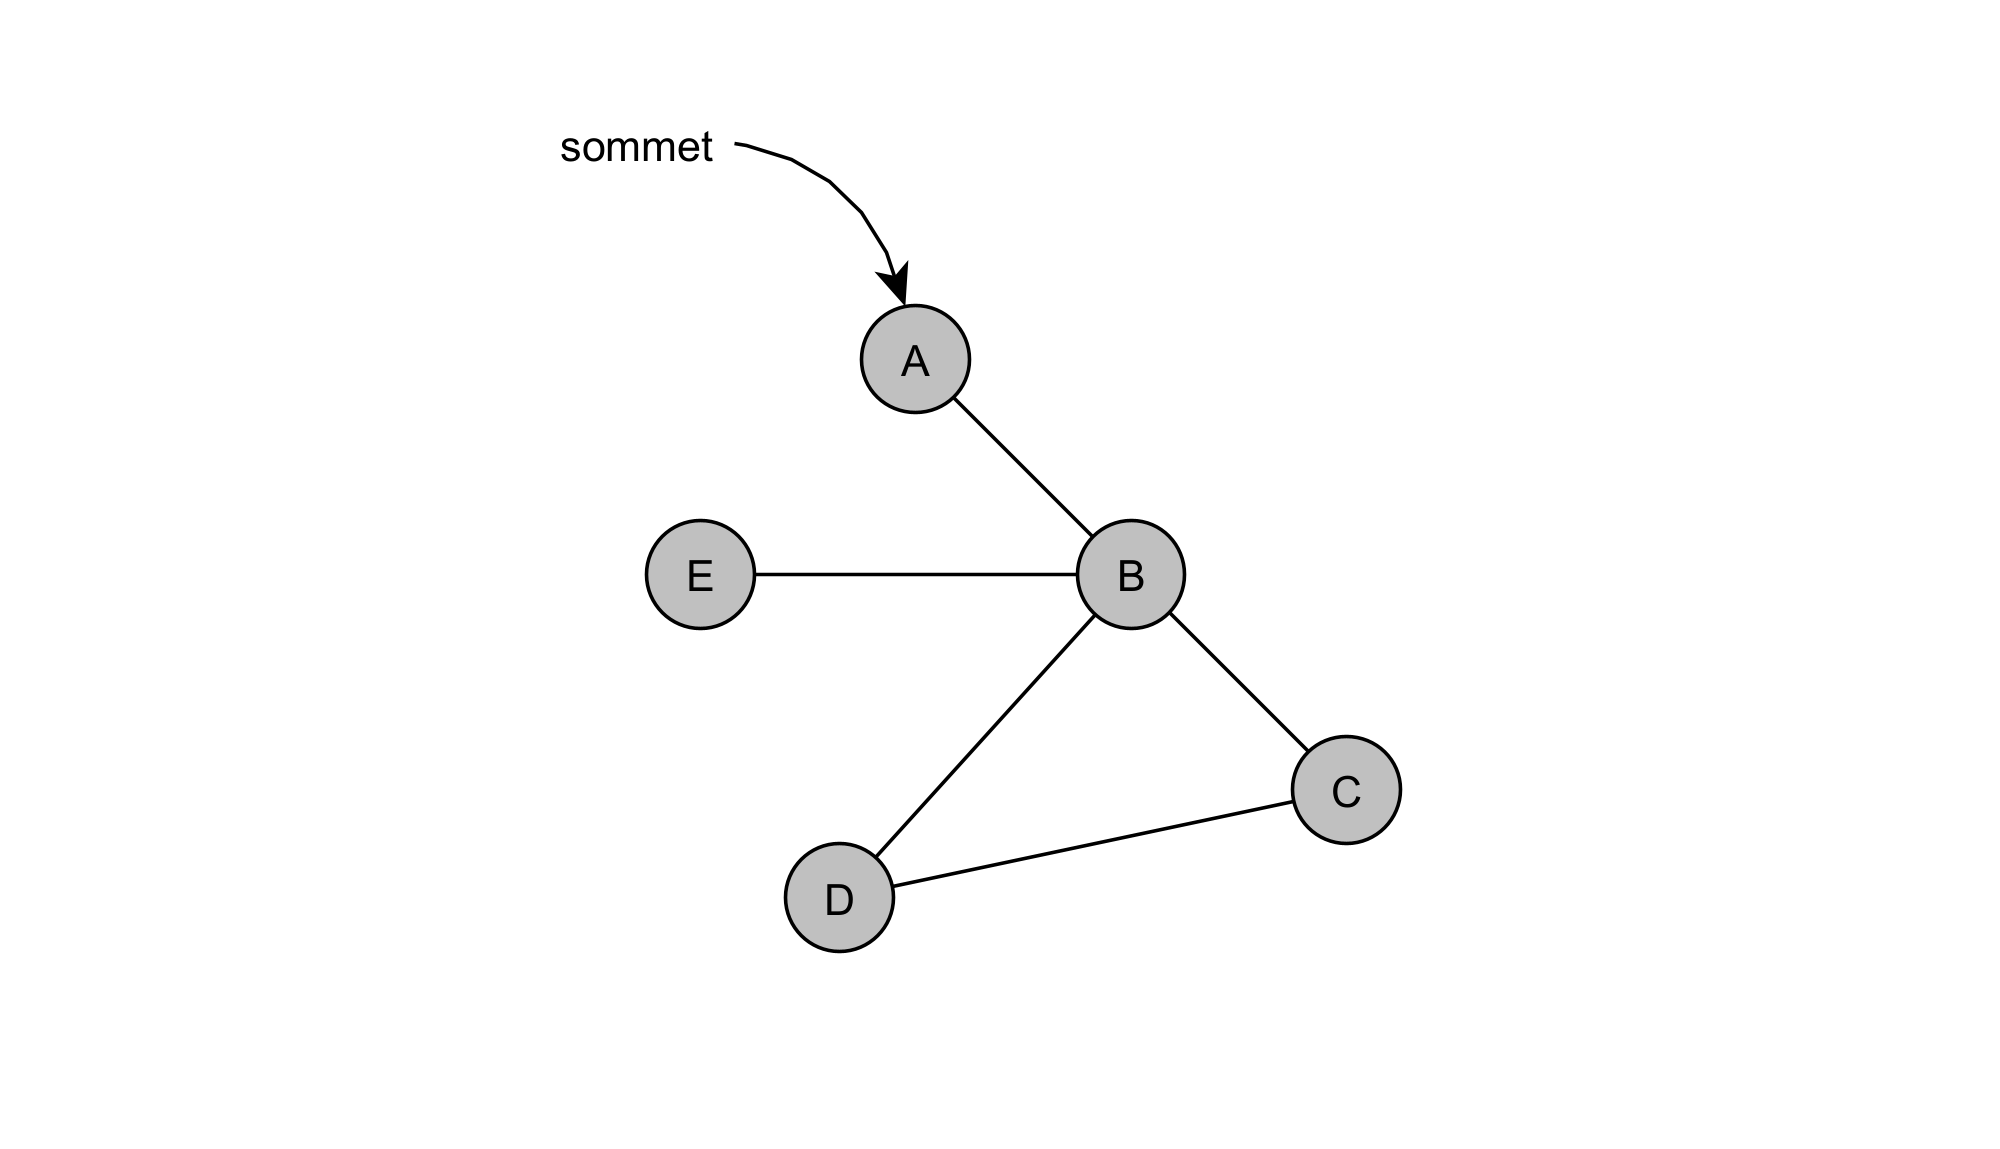
\includegraphics[width=9cm]{img/graph2}}
\only<2>{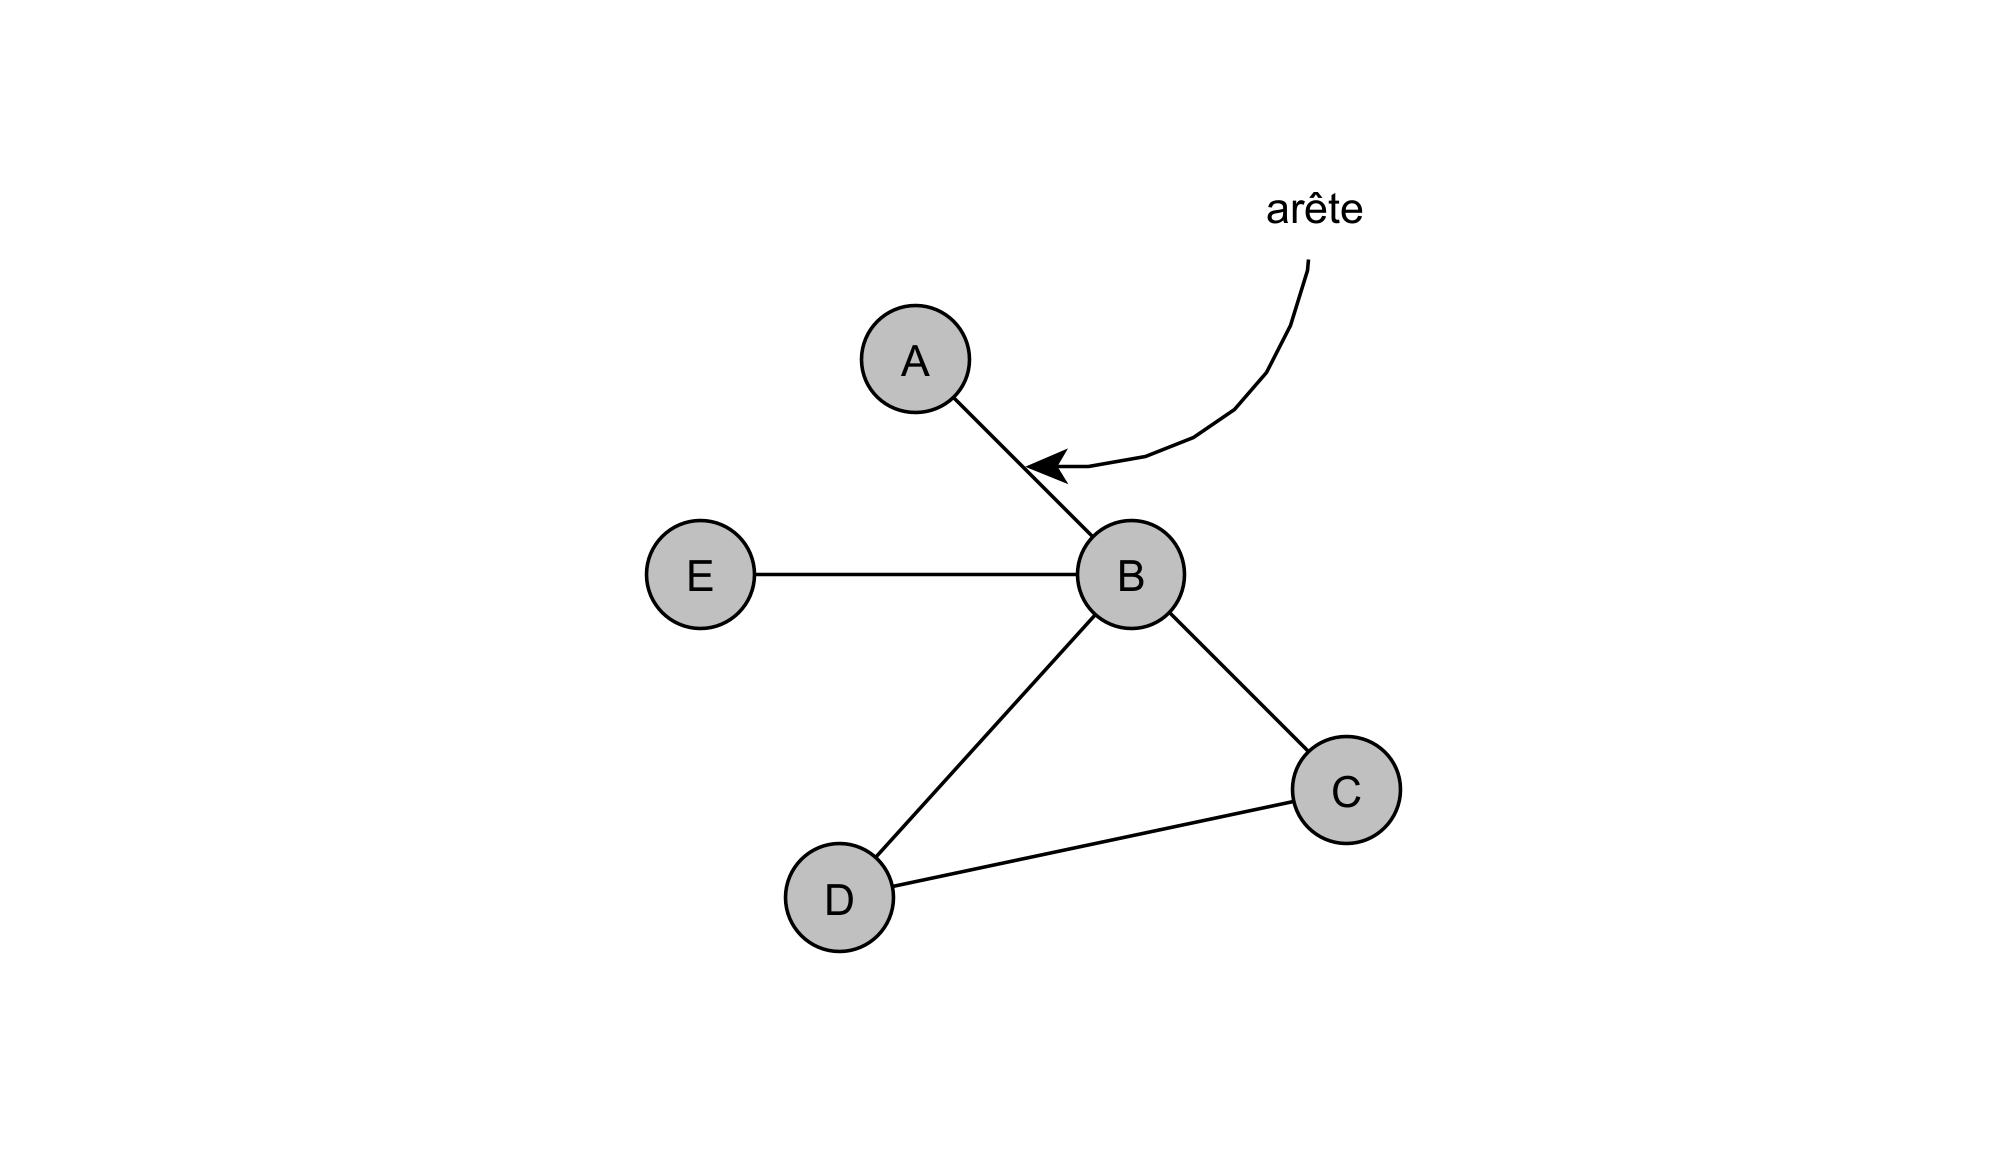
\includegraphics[width=9cm]{img/graph3}}
\only<3>{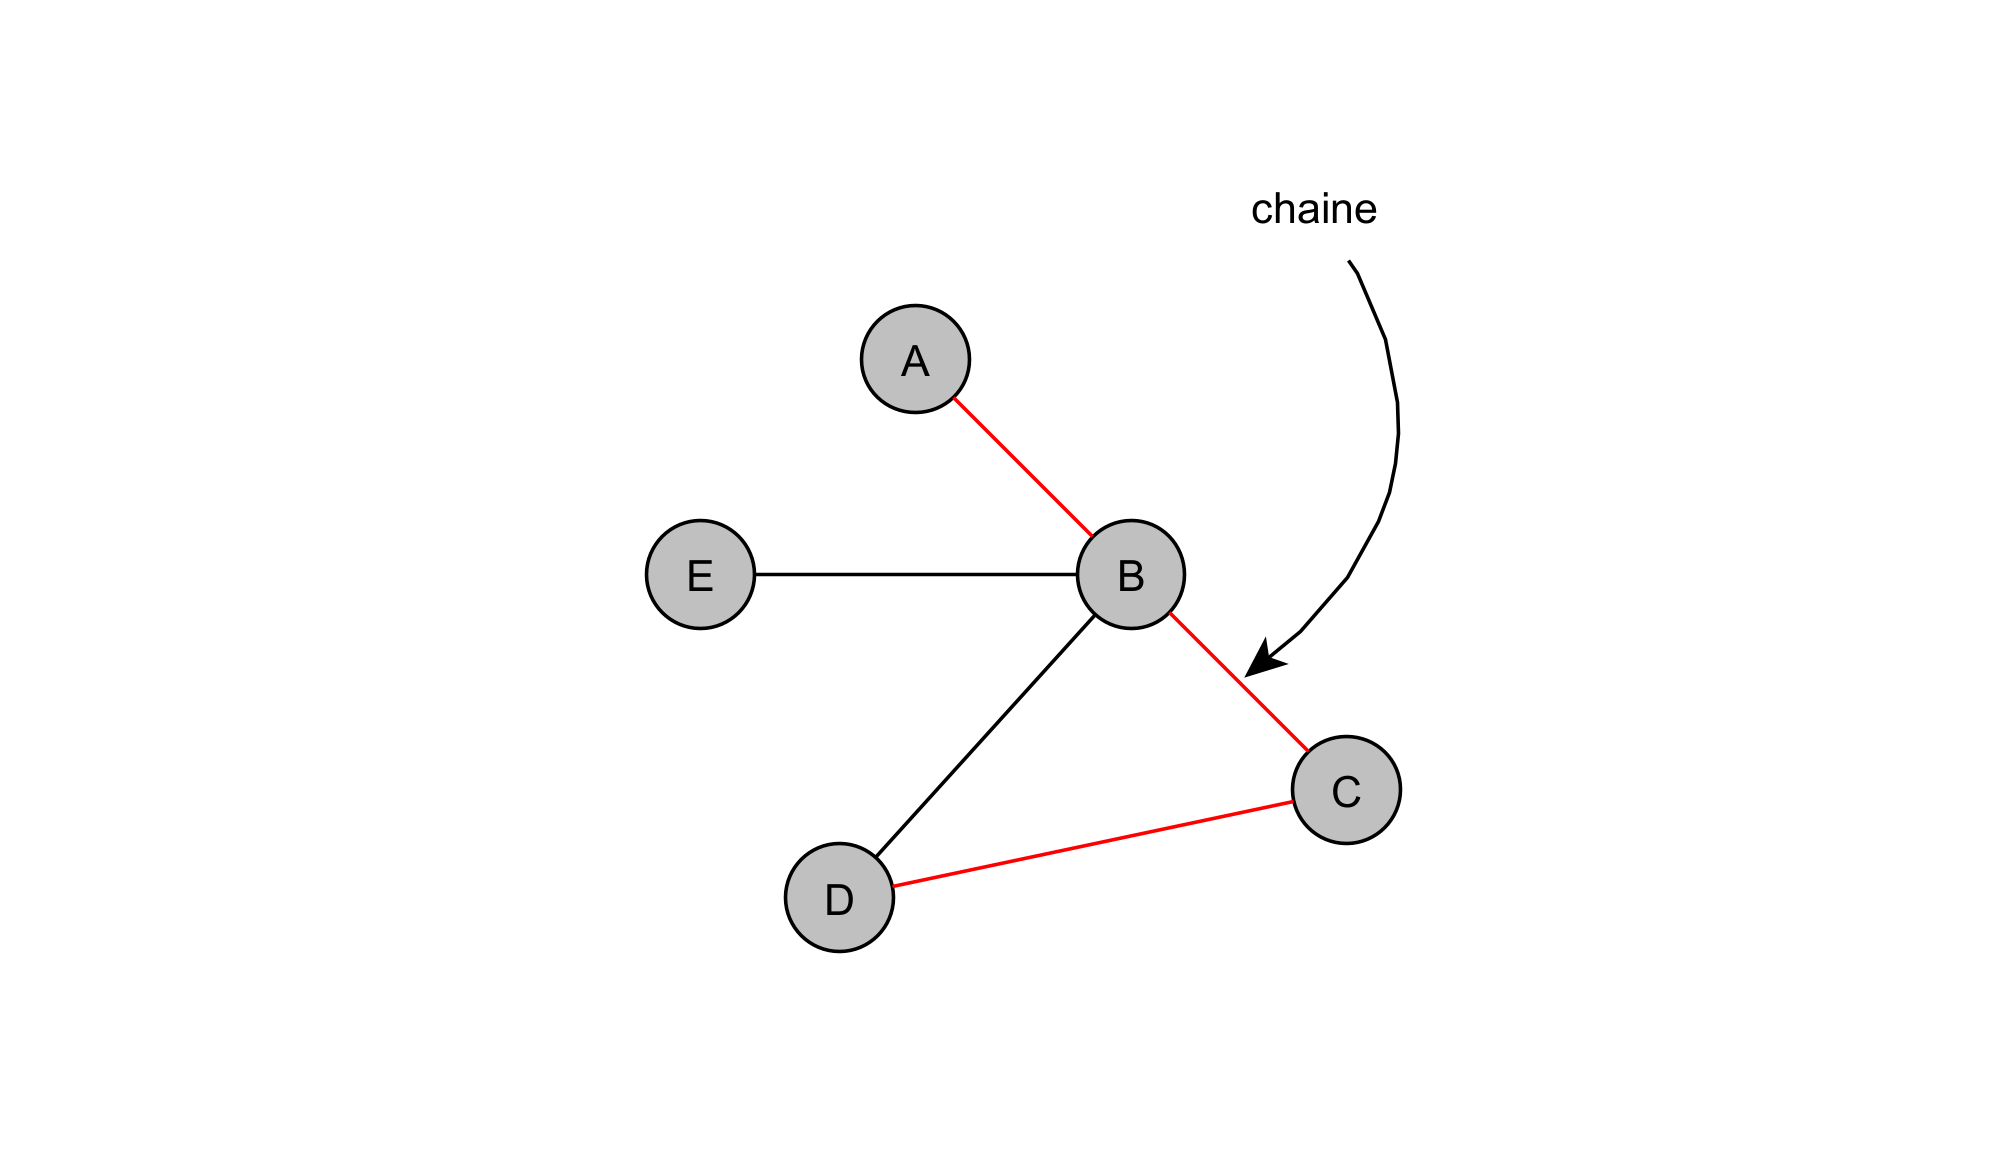
\includegraphics[width=9cm]{img/graph4}}
\only<4>{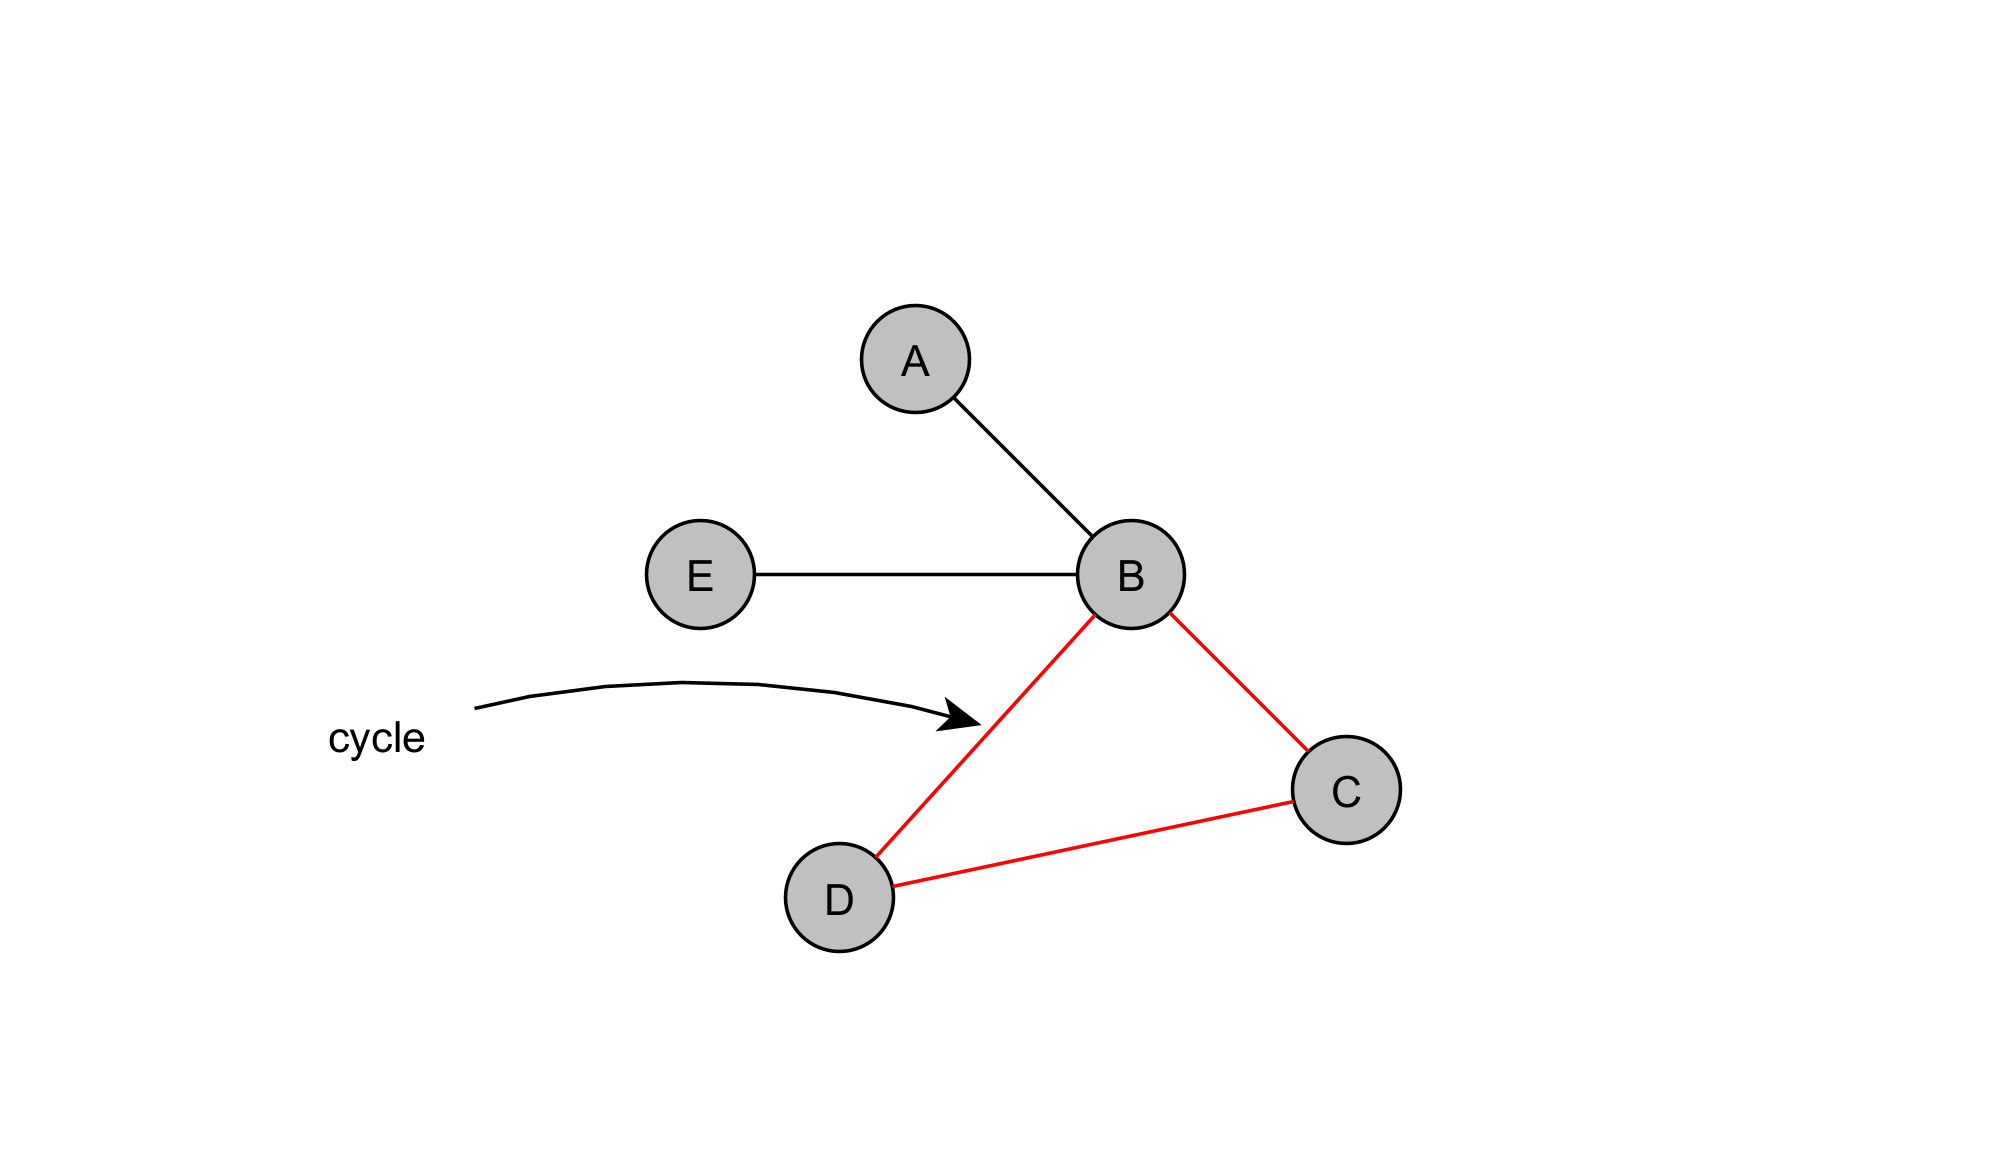
\includegraphics[width=9cm]{img/graph5}}
\end{center}
\end{frame}
\begin{frame}{Implémentations}
Comment peut-on implémenter une structure de graphe non-orienté ?\pause

Indice : le recyclage est conseillé...
\end{frame}

\section{Graphes pondérés}

\begin{frame}{Situation 1}
Encore une fois, pour faire simple, dans un \alert{graphe orienté pondéré} les arcs sont munis de poids qui sont en général des nombres réels strictement positifs.
\begin{center}
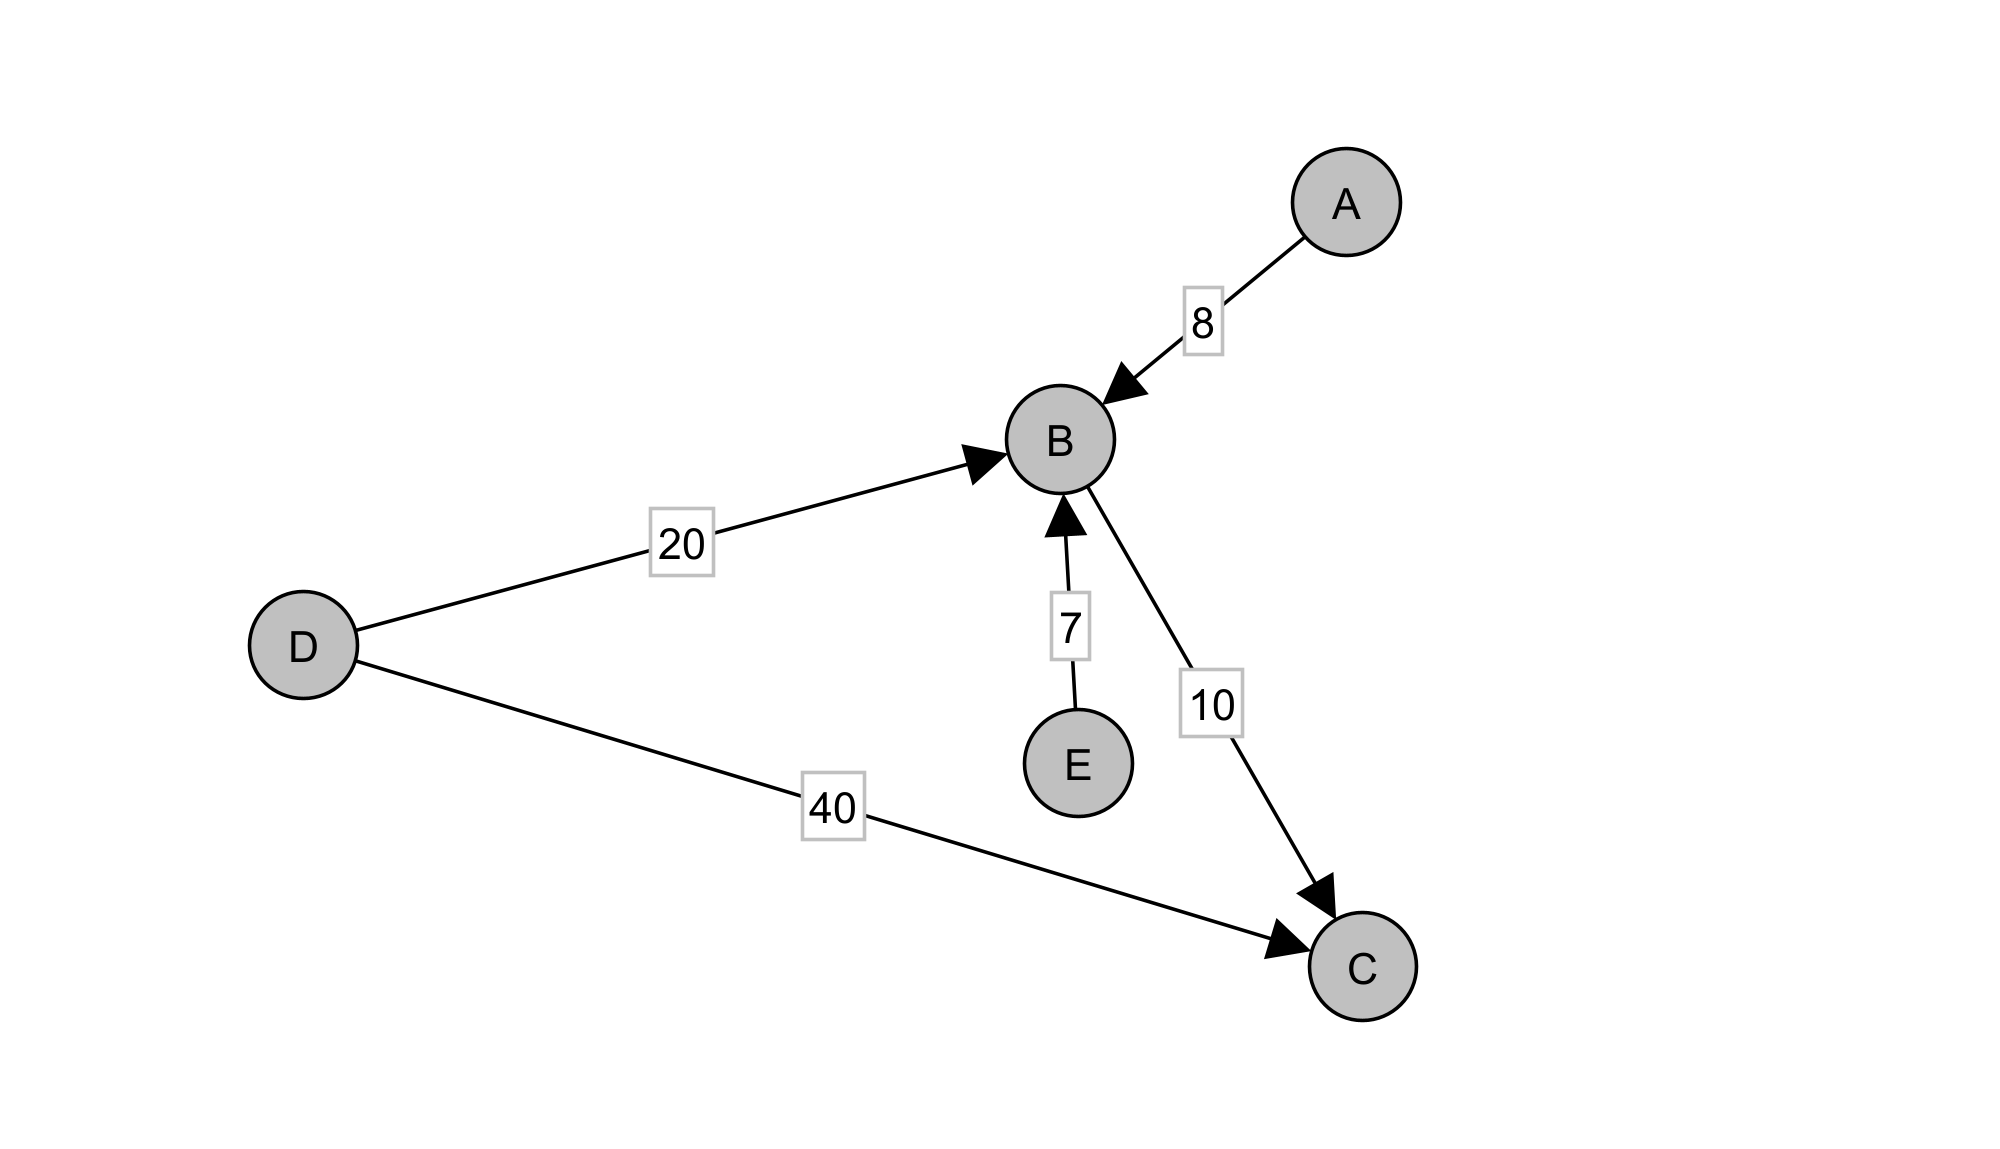
\includegraphics[width=9cm]{img/graphpo}
\end{center}
\end{frame}

\begin{frame}{Situation 2}
On rencontre également des \alert{graphes pondérés} (non orientés).
\begin{center}
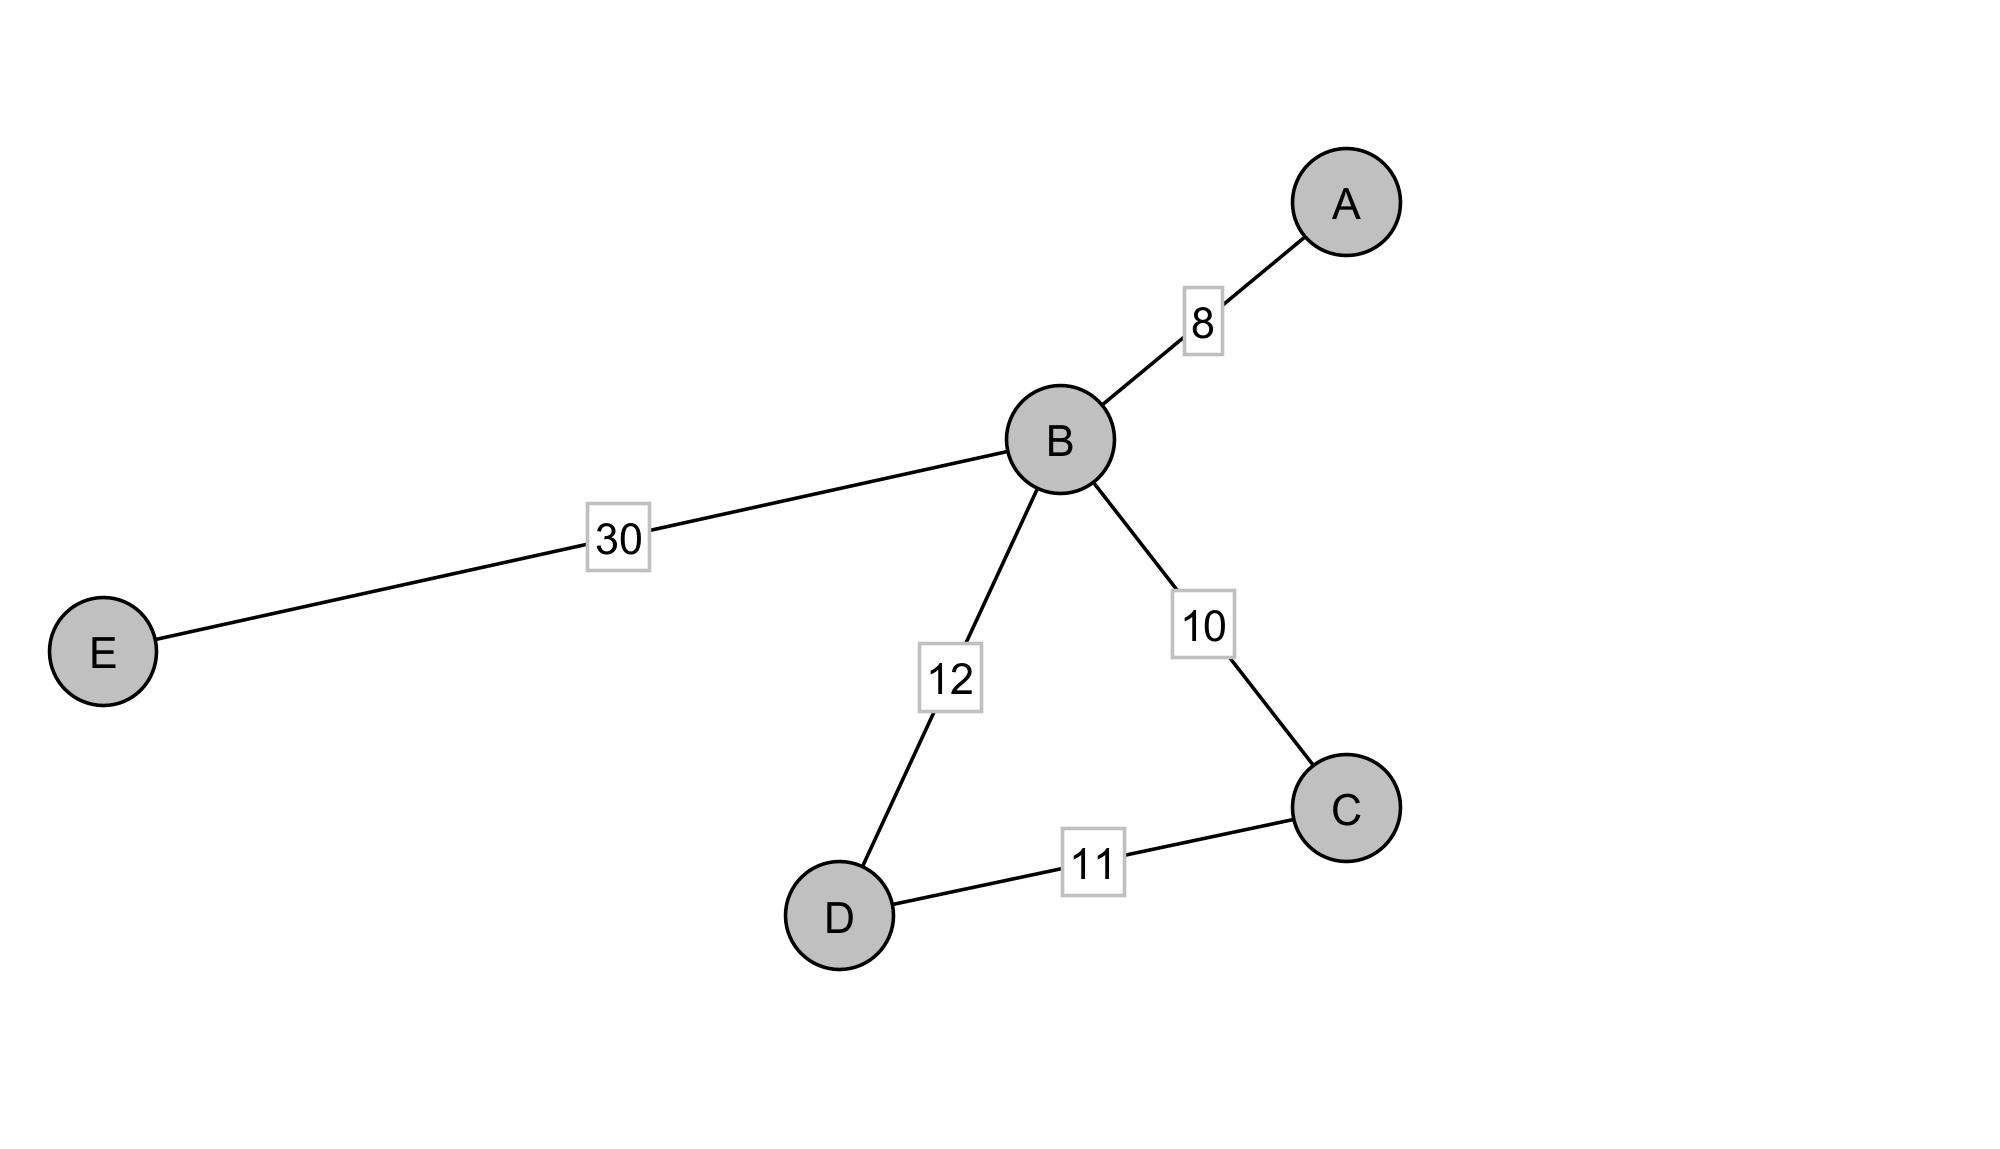
\includegraphics[width=9cm]{img/graphp}
\end{center}
\end{frame}

\begin{frame}{Implémentations}
Encore une fois se pose la question de l'implémentation de ses structures.\pause

Encore une fois le recyclage est conseillé...
\end{frame}

\section{Questions importantes}

\begin{frame}{Chemin ou chaîne}
\'Etant donné un graphe (orienté) et 2 sommets, existe-t-il une chaine (un chemin) reliant ces sommets ?
\begin{center}
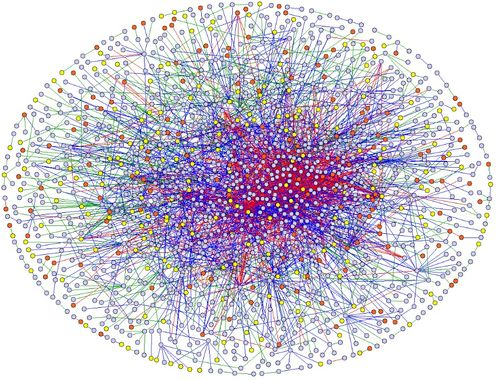
\includegraphics[width=8cm]{img/biggraph}
\end{center}
\end{frame}

\begin{frame}{Plus court chemin}
Quel est le plus court chemin entre 2 sommets d'un graphe pondéré ?
\begin{center}
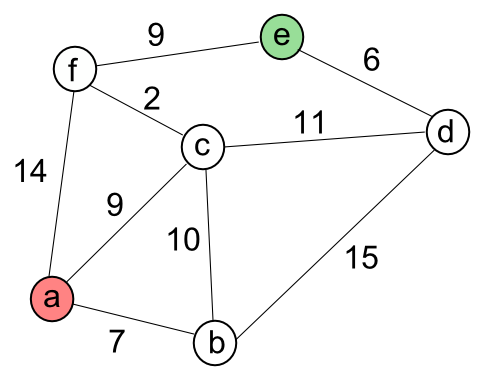
\includegraphics[width=9cm]{img/dijkstra}
\end{center}
\end{frame}

\begin{frame}{Coloration}
Combien faut-il de couleurs pour colorier les sommets d'un graphe sans que 2 voisins soient de la même couleur ?
\begin{center}
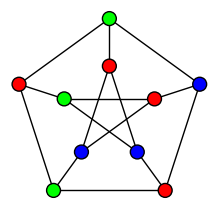
\includegraphics[width=7cm]{img/color}
\end{center}
\end{frame}

\begin{frame}{Applications}
Déterminer le routage des paquets dans un réseau.
\begin{center}
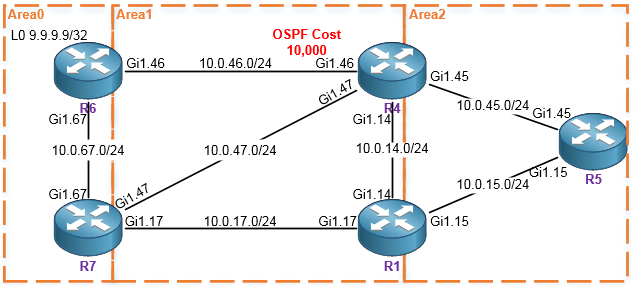
\includegraphics[width=9cm]{img/ospf}
\end{center}
\end{frame}

\begin{frame}{Applications}
Attribuer un minimum de fréquences à des antennes relais pour que le dispositif fonctionne sans interférences.
\begin{center}
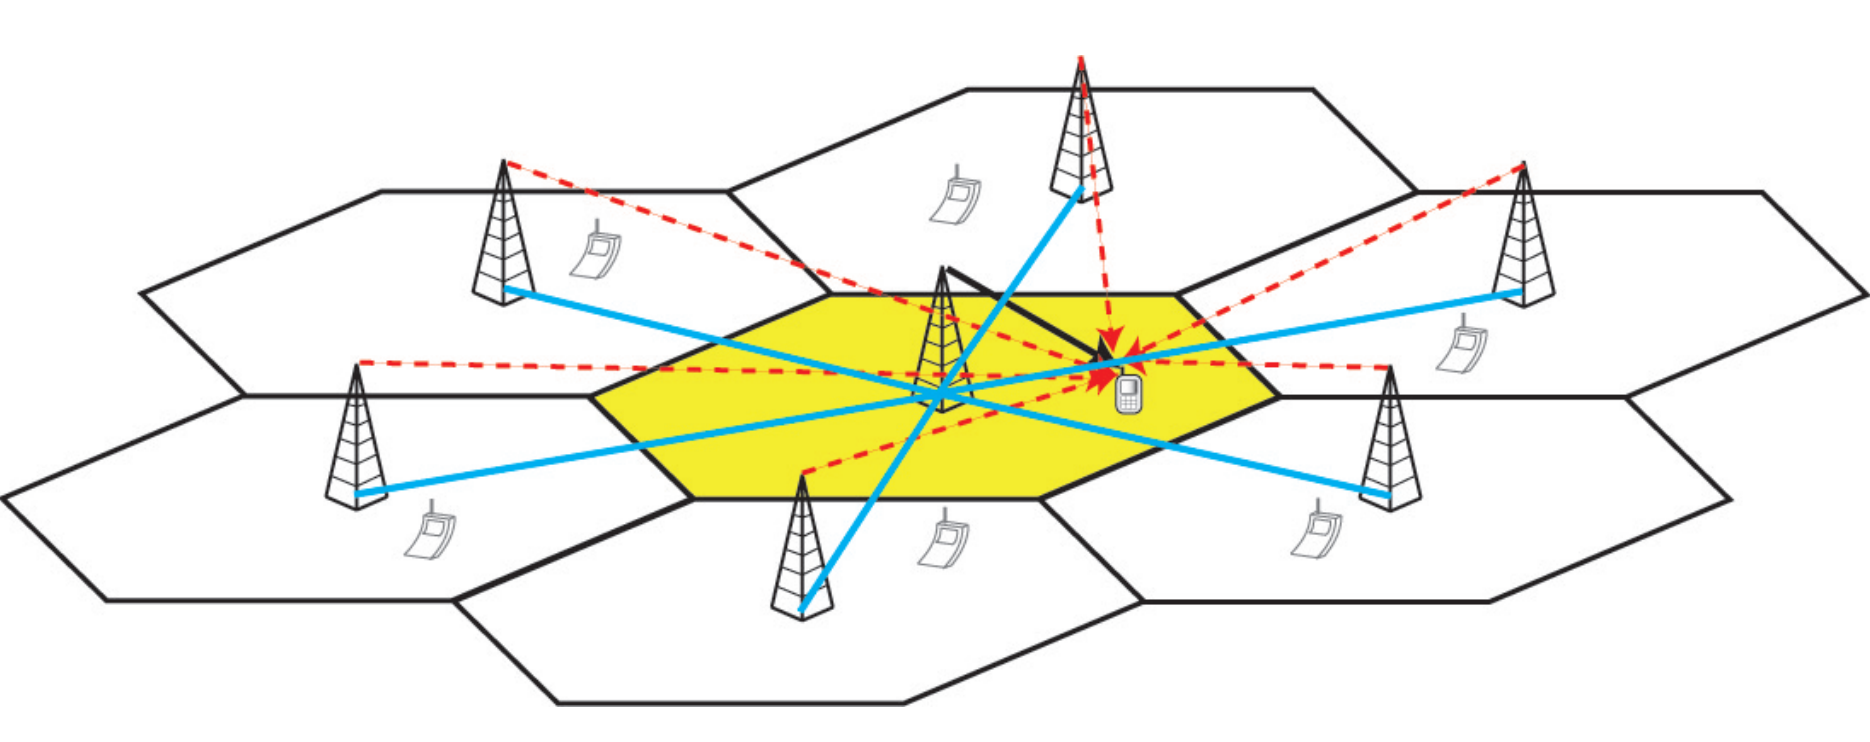
\includegraphics[width=9cm]{img/relais}
\end{center}
\end{frame}

\begin{frame}{Applications}
Attribuer un minimum de plages d'altitude à des vols pour que les normes de sécurité soient respectées.
\begin{center}
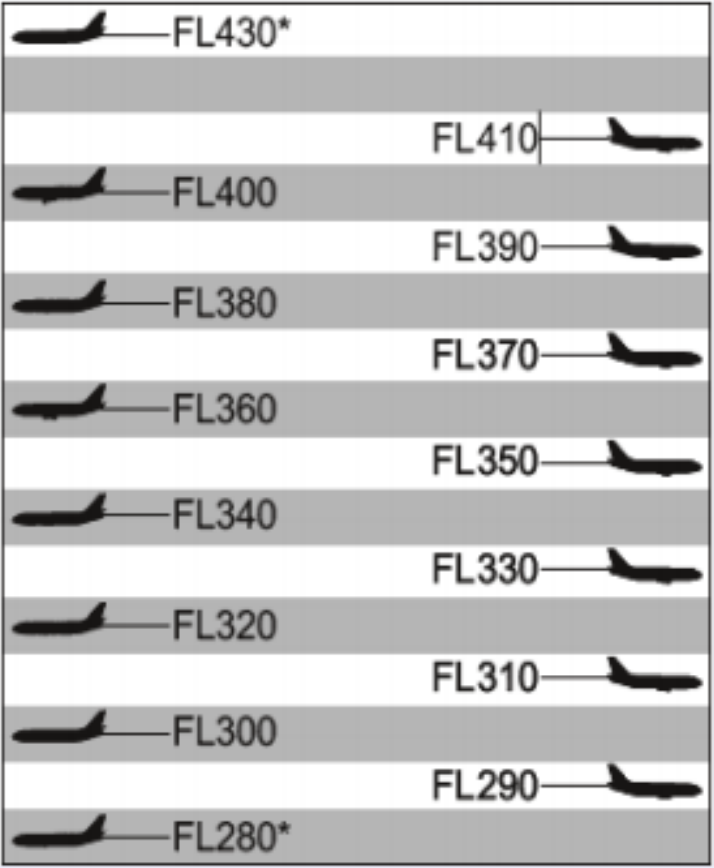
\includegraphics[width=5cm]{img/vols}
\end{center}
\end{frame}

\begin{frame}{Applications}
Déterminer si un début de sudoku est valide ou non.
\begin{center}
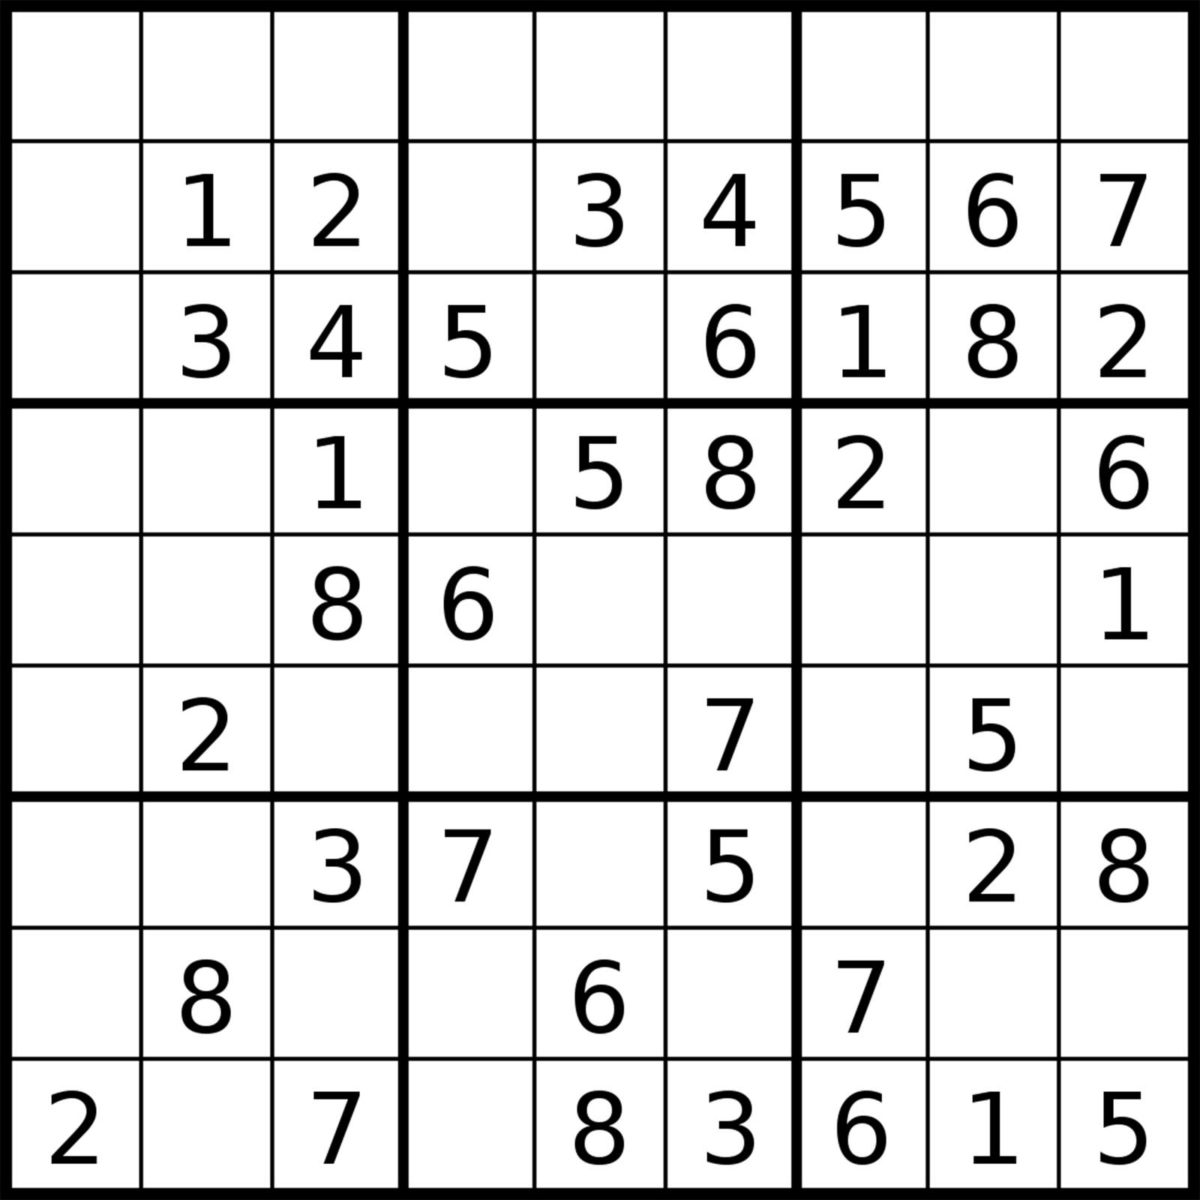
\includegraphics[width=7cm]{img/sudoku}
\end{center}
\end{frame}

\begin{frame}{Applications}
Composer des emplois du temps de manière efficace.
\begin{center}
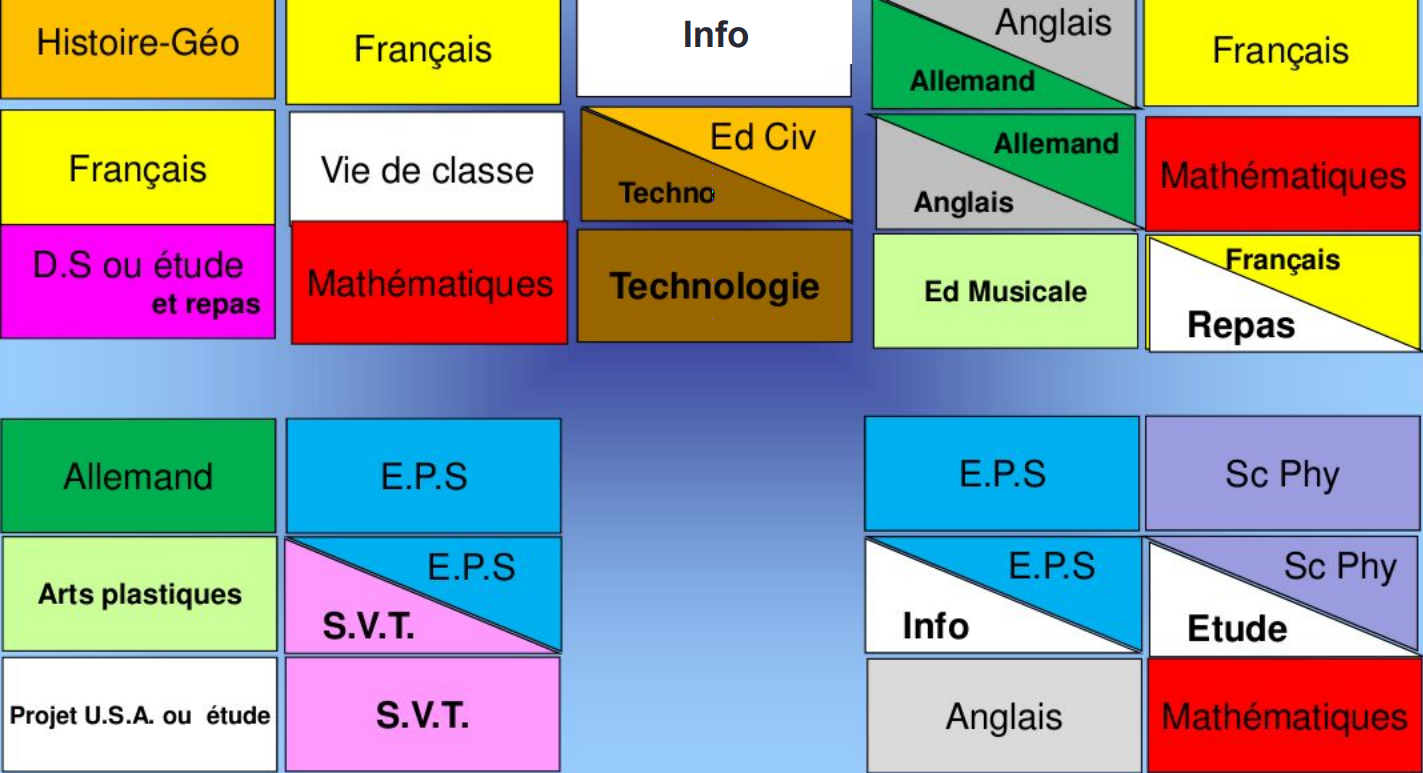
\includegraphics[width=9cm]{img/edt}
\end{center}
\end{frame}

\end{document}